% ============================================================
% APPENDICE A - APPROFONDIMENTI «CON LA FISICA» E «CON LA MATEMATICA»
% ============================================================
\appendix

\chapter{Approfondimenti «Con la fisica» e «Con la matematica»}
\chaptermark{Approfondimenti}
\label{app:approfondimenti}

Questi box raccolgono le spiegazioni fisiche e matematiche citate nei capitoli. Sono facoltativi: il percorso principale non dipende da essi. Ogni capitolo rimanda al box che lo riguarda.

\section*{Suono e triadi}

\begin{fisica}[La serie degli armonici come fondamento fisico della tonalità]
	\label{phys:serie_armonici_fondamento}

	Un suono musicale non è una singola frequenza. Partiamo dall'equazione delle \textbf{onde stazionarie}: quando una corda vibrante o una colonna d'aria sono vincolate ai loro estremi, possono vibrare solo secondo particolari modi, i \textbf{modi normali di vibrazione}.

	La condizione fisica per questi modi è che la lunghezza della corda $L$ contenga un numero intero di mezze lunghezze d'onda:
	\[
	L = n \cdot \frac{\lambda_n}{2} \quad \text{con } n = 1, 2, 3, \ldots
	\]

	Usando la relazione fondamentale tra velocità, frequenza e lunghezza d'onda ($v = \lambda \cdot f$) si ottengono le frequenze dei modi possibili:
	\[
	f_n = n \cdot f_1 = n \cdot \frac{v}{2L}
	\]

	dove $f_1$ è la \textbf{frequenza fondamentale} (primo armonico) e $f_n$ sono gli \textbf{armonici superiori}. Ne segue che:
	\begin{itemize}
		\item il secondo armonico ha frequenza $2f_1$ (un'ottava sopra la fondamentale);
		\item il terzo armonico ha frequenza $3f_1$ (una quinta giusta sopra l'ottava);
		\item il quarto armonico ha frequenza $4f_1$ (due ottave sopra);
		\item il quinto armonico ha frequenza $5f_1$ (una terza maggiore sopra le due ottave).
	\end{itemize}

	\textbf{Rapporti di frequenza e intervalli musicali}

	\begin{itemize}
		\item \textbf{Ottava}: $\frac{f_2}{f_1} = \frac{2f_1}{f_1} = 2:1$
		\item \textbf{Quinta giusta}: $\frac{f_3}{f_2} = \frac{3f_1}{2f_1} = 3:2$
		\item \textbf{Terza maggiore}: $\frac{f_5}{f_4} = \frac{5f_1}{4f_1} = 5:4$
	\end{itemize}

	Questi rapporti tra numeri interi piccoli (2:1, 3:2, 5:4) sono quelli che l'orecchio percepisce come più \textbf{consonanti} e \textbf{stabili}. La fisica delle onde stazionarie spiega quindi perché l'accordo maggiore, costruito con questi intervalli, sia la base naturale del sistema tonale.

	\textbf{Conseguenze per la teoria armonica}

	La serie armonica spiega perché:
	\begin{enumerate}
		\item la quinta giusta (3:2) appare prima della terza maggiore (5:4) nella serie: la quinta è un intervallo più «fondamentale»;
		\item l'accordo maggiore (Do-Mi-Sol) ha rapporti 4:5:6: sono il quarto, il quinto e il sesto armonico della stessa fondamentale;
		\item gli intervalli con rapporti più complessi, come il tritono, sono percepiti come più dissonanti.
	\end{enumerate}
\end{fisica}

\begin{matematica}[L'aritmetica modulare come «orologio» del sistema tonale]
	\label{math:aritmetica_modulare}

	Il sistema tonale occidentale divide l'ottava in 12 semitoni, in una struttura che si ripete identica a ogni ottava. Questa natura \textbf{ciclica} si descrive con l'\textbf{aritmetica modulare}, la stessa matematica con cui si legge l'orologio.

	\textbf{L'insieme $\mathbb{Z}_{12}$}

	Si associa a ogni nota una classe di altezza, un numero da 0 a 11:
	\[
	\begin{array}{cccccccccccc}
	\text{Do} & \text{\Dodiesis } & \text{Re} & \text{\Rediesis } & \text{Mi} & \text{Fa} & \text{\Fadiesis } & \text{Sol} & \text{\Soldiesis } & \text{La} & \text{\Ladiesis } & \text{Si} \\
	0 & 1 & 2 & 3 & 4 & 5 & 6 & 7 & 8 & 9 & 10 & 11
	\end{array}
	\]

	L'insieme $\mathbb{Z}_{12} = \{0, 1, 2, \ldots, 11\}$ con l'\textbf{addizione modulo 12} è un \textbf{gruppo ciclico}. Come per l'orologio, quando si supera 11 si «torna indietro» a 0:
	\[
	a +_{12} b = (a + b) \mod 12
	\]

	\textbf{Calcolo di intervalli}

	\begin{itemize}
		\item \textbf{Quinta giusta ascendente} (7 semitoni).\\
		Da Do (0) a Sol: $0 + 7 = 7$ (Sol)\\
		Da Mi (4) a Si: $4 + 7 = 11$ (Si)\\
		Da Sol (7) a Re: $7 + 7 = 14 \equiv 2 \pmod{12}$ (Re)

		\item \textbf{Trasposizione}: trasporre di una terza maggiore (4 semitoni) significa sommare 4 a ogni nota.\\
		Accordo di Do maggiore: $(0, 4, 7)$ diventa $(4, 8, 11)$ = Mi maggiore
	\end{itemize}

	\textbf{Il circolo delle quinte come sequenza algoritmica}

	Il circolo delle quinte nasce da una \textbf{funzione ricorsiva}:
	\[
	x_{n+1} = (x_n + 7) \mod 12
	\]

	Da Do ($x_0 = 0$):
	\begin{align*}
	x_1 &= (0 + 7) \mod 12 = 7 \quad \text{(Sol)} \\
	x_2 &= (7 + 7) \mod 12 = 2 \quad \text{(Re)} \\
	x_3 &= (2 + 7) \mod 12 = 9 \quad \text{(La)} \\
	x_4 &= (9 + 7) \mod 12 = 4 \quad \text{(Mi)} \\
	&\vdots
	\end{align*}

	Dopo 12 iterazioni si torna a 0 (Do): il circolo delle quinte discende dall'aritmetica del sistema a 12 semitoni.

	\textbf{Proprietà}

	\begin{itemize}
		\item L'operazione «+7» genera tutti i 12 elementi di $\mathbb{Z}_{12}$ perché 7 e 12 sono \textbf{coprimi} ($\text{MCD}(7, 12) = 1$).
		\item Il circolo delle quarte si ottiene con l'operazione inversa: $x_{n+1} = (x_n + 5) \mod 12$, equivalente a $x_{n+1} = (x_n - 7) \mod 12$.
		\item La simmetria enarmonica (\Fadiesis  = \Solbemolle ) corrisponde a $6 + 6 = 12 \equiv 0 \pmod{12}$: il tritono divide l'ottava esattamente a metà.
	\end{itemize}

	Gli stessi calcoli sono usati dai programmi musicali per trasporre le note e analizzare le progressioni armoniche.
\end{matematica}

\begin{fisica}[I rapporti di frequenza e la stabilità degli accordi]
	\label{phys:rapporti_frequenza_triadi}

	Per capire perché alcune triadi suonano più stabili di altre si analizzano i rapporti di frequenza tra le loro note.

	\textbf{La triade maggiore e i rapporti semplici}

	Si consideri la triade di Do maggiore (Do-Mi-Sol), con il Do a frequenza $f_1$. Le frequenze approssimate nella scala temperata sono:
	\begin{itemize}
		\item Do (fondamentale): $f_1$
		\item Mi (terza maggiore): $\approx 1{,}26 \cdot f_1$ (rapporto ideale $5:4 = 1{,}25$)
		\item Sol (quinta giusta): $\approx 1{,}50 \cdot f_1$ (rapporto ideale $3:2 = 1{,}50$)
	\end{itemize}

	Nell'intonazione naturale (o «giusta») i rapporti sono esatti: $4:5:6$. Se il Do vibra a 200 Hz, il Mi vibra a 250 Hz e il Sol a 300 Hz. Il rapporto tra \textbf{numeri interi piccoli} è ciò che l'orecchio percepisce come massimamente consonante.

	\textbf{La triade diminuita e i rapporti complessi}

	Per la triade diminuita (Do-\Mibemolle -\Solbemolle ) i rapporti approssimati sono:
	\begin{itemize}
		\item Do: $f_1$
		\item \Mibemolle  (terza minore): $\approx 1{,}19 \cdot f_1$ (rapporto $6:5$)
		\item \Solbemolle  (quinta diminuita): $\approx 1{,}41 \cdot f_1$ (rapporto complesso, circa $\sqrt{2}:1$)
	\end{itemize}

	Il \textbf{tritono} (Do-\Solbemolle{}, rapporto $\sqrt{2}:1$ nel temperamento equabile) non si esprime come rapporto di numeri interi piccoli, perché $\sqrt{2}$ è irrazionale. Approssimandolo si ottiene qualcosa come $45:32$ o $64:45$, numeri molto più grandi.

	\textbf{I battimenti acustici}

	Quando due frequenze vicine suonano insieme, si genera un \textbf{battimento} di frequenza pari alla differenza:
	\[
	f_{\text{battimento}} = |f_2 - f_1|
	\]

	Con rapporti semplici (come 3:2) gli armonici delle due note tendono a coincidere o a stare molto distanti, e i battimenti sono minimi. Con rapporti complessi molti armonici cadono vicini ma non coincidenti, e i battimenti multipli sono percepiti come «ruvidità», cioè come \textbf{dissonanza}.

	\begin{center}
	\begin{tabular}{lcl}
	\toprule
	\textbf{Triade} & \textbf{Rapporti (ideali)} & \textbf{Percezione} \\
	\midrule
	Maggiore & $4:5:6$ & stabile, luminosa \\
	Minore & $10:12:15$ & stabile, malinconica \\
	Diminuita & include il tritono & instabile, tesa \\
	Eccedente & include la 5a aumentata & ambigua, irrequieta \\
	\bottomrule
	\end{tabular}
	\end{center}
\end{fisica}

\begin{fisica}[Il conflitto acustico dell'accordo di quarta e sesta]
	\label{phys:conflitto_6_4}

	Ascoltando un accordo, l'orecchio tende a identificare la nota più grave (il basso reale) come fondamentale «percepita», perché la nota al basso genera la propria serie armonica, che domina la percezione complessiva.

	\textbf{Il conflitto della quarta}

	Nel secondo rivolto la fondamentale dell'accordo sta a distanza di \textbf{quarta} dal basso. La fondamentale (rapporto $4:3$ con il basso) non compare tra i primi armonici della serie del basso: l'orecchio sente il basso come fondamentale, mentre la struttura dell'accordo ne indica un'altra, e questa ambiguità rende l'accordo instabile.

	\textbf{Rappresentazione matematica}

	Se il basso suona a frequenza $f_b$, i suoi armonici principali sono $f_b$, $2f_b$, $3f_b$, $4f_b$, $5f_b$\ldots La quarta sopra il basso ha frequenza $f_4 = \frac{4}{3}f_b$, che non appare tra i primi armonici semplici, mentre la quinta ($3:2$) è il secondo rapporto più consonante dopo l'ottava.

	L'accordo di 6/4 è dissonante per la disposizione delle note, non per le note in sé: per questo richiede sempre un trattamento particolare.
\end{fisica}

\section*{Funzioni e Regola dell'Ottava}

\begin{matematica}[L'identità del III grado: tra tonica e dominante]
	\label{math:identita_iii}
	La parentela fra gli accordi si può analizzare con la teoria degli insiemi. Le triadi di Do maggiore come insiemi di note sono:
	\begin{itemize}
		\item $\text{I} = \{\text{Do}, \text{Mi}, \text{Sol}\}$
		\item $\text{III} = \{\text{Mi}, \text{Sol}, \text{Si}\}$
		\item $\text{V} = \{\text{Sol}, \text{Si}, \text{Re}\}$
	\end{itemize}
	La cardinalità dell'intersezione è identica nei due casi: $|\text{I} \cap \text{III}| = 2$ (Mi, Sol) e $|\text{V} \cap \text{III}| = 2$ (Sol, Si).

	Perché il III grado è allora una «tonica debole» e non una dominante? Conta la \textbf{gerarchia pesata} degli elementi:
	\begin{enumerate}
		\item Il Mi è la \textit{caratteristica modale} della tonica; la sua presenza nel III grado stabilisce un legame forte con la «casa» della tonalità.
		\item Il III grado contiene la sensibile (Si) ma non la \textit{fondamentale} della dominante (Sol al basso o come nota portante), necessaria per la spinta verso la risoluzione.
	\end{enumerate}
	Pur avendo lo stesso numero di note in comune con il V grado, prevale la «forza gravitazionale» delle note in comune con il I grado, e il III grado sostituisce il riposo e non la tensione.
\end{matematica}

\begin{fisica}[Perché il \sigla{I}{6}{4} sul V grado suona «sospeso»]
	\label{phys:i64_sospeso}
	Suonando il secondo rivolto della tonica (\sigla{I}{6}{4}) con il Sol al basso (V grado in Do maggiore), le note sono Sol-Do-Mi. Acusticamente:

	\begin{itemize}
		\item la quarta Sol-Do ha rapporto di frequenza 4:3;
		\item questo rapporto non appare tra i primi armonici semplici del basso (Sol);
		\item gli armonici di Sol sono Sol, Sol, Re, Sol, Si, Re\ldots ma non Do;
		\item il Do risulta quindi «estraneo» alla serie armonica naturale del basso.
	\end{itemize}

	Questa estraneità acustica genera l'instabilità e la sospensione che caratterizzano il \sigla{I}{6}{4}. Quando risolve sul V (Sol-Si-Re-Fa), la quarta Sol-Do scende alla terza Sol-Si, che è invece il quinto armonico del basso: la risoluzione è acusticamente «naturale». È la ragione fisica per cui il secondo rivolto, pur essendo tecnicamente un accordo di tonica, funziona come preparazione della dominante.
\end{fisica}

\section*{Settime}

\begin{fisica}[I battimenti e la tensione del tritono]
	\label{phys:battimenti_tritono}

	Il tritono è l'intervallo più dissonante del sistema diatonico. La «ruvidità» che si percepisce ha una base fisica nei \textbf{battimenti acustici}.

	\textbf{Cosa sono i battimenti}

	Quando due onde con frequenze vicine ma non identiche suonano insieme si ha \textbf{interferenza}: le onde si sommano alternando momenti costruttivi (si rafforzano) e distruttivi (si attenuano). L'intensità fluttua periodicamente, come un «tremolo» detto \textbf{battimento}, la cui frequenza è la differenza fra le due:
	\[
	f_{\text{battimento}} = |f_2 - f_1|
	\]

	\textbf{Il tritono e i battimenti multipli}

	Nel temperamento equabile il tritono Si-Fa ha:
	\begin{itemize}
		\item Si: frequenza $f_1$
		\item Fa: frequenza $f_2 \approx 1{,}414 f_1$ (rapporto $\sqrt{2}:1$, cioè 6 semitoni)
	\end{itemize}

	Il rapporto $\sqrt{2}:1$ è \textbf{irrazionale}. Gli armonici di Si sono $f_1, 2f_1, 3f_1, 4f_1, 5f_1, \ldots$, quelli di Fa $1{,}414f_1, 2{,}828f_1, 4{,}243f_1, 5{,}657f_1, \ldots$ e non coincidono mai, ma cadono in posizioni intermedie:
	\begin{itemize}
		\item $2f_1$ contro $2{,}828f_1$: differenza $\approx 0{,}828f_1$
		\item $4f_1$ contro $4{,}243f_1$: differenza $\approx 0{,}243f_1$
	\end{itemize}

	Ogni coppia di armonici vicini ma non coincidenti genera il proprio battimento. Il risultato è una \textbf{ruvidità acustica complessa}, che si identifica con la dissonanza.

	\textbf{Confronto con un intervallo consonante}

	La quinta giusta (Sol-Re in Do maggiore) ha rapporto $3:2$, razionale e semplice: il 3° armonico di Sol coincide con il 2° armonico di Re. Ci sono pochi battimenti, e il suono è «pulito» e stabile.

	\textbf{La risoluzione come riduzione dei battimenti}

	Quando la \sigla{V}{7}{} risolve sulla tonica il tritono si muove verso intervalli più consonanti: Si $\rightarrow$ Do (la sensibile sale), Fa $\rightarrow$ Mi (la settima scende). Il tritono Si-Fa diventa la terza Do-Mi o la sesta Mi-Do. Il movimento è una \textbf{transizione da rapporti complessi a rapporti semplici}, da molti battimenti a pochi: l'orecchio la percepisce come passaggio dalla tensione al riposo.
\end{fisica}

\begin{fisica}[La doppia tensione della \sigla{V}{7}{} nel modo minore]
	\label{phys:doppia_tensione_v7}
	Nel modo minore la settima di dominante (per esempio Mi-\Soldiesis -Si-Re in La minore) ha un'intensità particolare. La sensibile alterata (\Soldiesis) è attratta di semitono verso il La, la settima (Re) scende verso il Do, e fra le due c'è la quinta diminuita \Soldiesis -Re, un tritono.

	Il tritono produce \textbf{battimenti} percepibili per la vicinanza dei suoi armonici superiori; il suo rapporto temperato ($2^{6/12} = \sqrt{2} \approx 1{,}414$) non corrisponde a nessun rapporto semplice. Questa «rugosità», sommata alle due tensioni melodiche opposte (\Soldiesis  verso l'alto, Re verso il basso), spiega perché la \sigla{V}{7}{} del modo minore suona così drammatica e chiede la risoluzione sulla tonica.
\end{fisica}

\begin{matematica}[Crescita combinatoria delle possibilità armoniche]
	\label{math:crescita_combinatoria}
	Come cresce la complessità passando da una versione all'altra della Regola dell'Ottava:

	\textbf{Versione preliminare:}
	\begin{itemize}
		\item 7 triadi diatoniche, 3 stati per ciascuna (fondamentale e due rivolti);
		\item $7 \times 3 = 21$ configurazioni di base.
	\end{itemize}

	\textbf{Versione intermedia:}
	\begin{itemize}
		\item le 21 precedenti, più un accordo di settima (\sigla{V}{7}{}) con 4 stati;
		\item $21 + 4 = 25$ configurazioni.
	\end{itemize}

	\textbf{Versione completa:}
	\begin{itemize}
		\item le precedenti, più 6 nuove settime diatoniche (\sigla{I}{7}{}, \sigla{II}{7}{}, \sigla{III}{7}{}, \sigla{IV}{7}{}, \sigla{VI}{7}{}, \sigla{VII}{7}{}) con 4 stati ciascuna;
		\item totale teorico: $21 + (7 \times 4) = 49$ configurazioni.
	\end{itemize}

	La versione completa offre più del doppio delle possibilità della preliminare.
\end{matematica}

\begin{fisica}[Perché le settime «colorano» l'armonia]
	\label{phys:settime_colore}
	Gli intervalli di settima creano battimenti tra gli armonici parziali e rendono la trama sonora più densa. Le note di una triade tendono a fondersi; quelle di un accordo di settima restano più separate all'ascolto e danno un senso di «movimento interno». La dissonanza di settima, infine, fa attendere una risoluzione e guida l'orecchio verso accordi precisi.
\end{fisica}

\section*{Progressioni}

\begin{fisica}[Perché le progressioni funzionano]
	\label{phys:perche_progressioni}
	Dal punto di vista percettivo le progressioni sfruttano il \textbf{riconoscimento di schemi}. Dopo una o due ripetizioni del modello l'ascoltatore anticipa il movimento successivo e segue senza fatica la struttura complessiva. Per questo le progressioni danno varietà armonica senza disorientare l'ascolto.
\end{fisica}

\begin{fisica}[La «fisica» delle progressioni: energia armonica]
	\label{phys:energia_armonica}
	Si può pensare alle progressioni in termini di \textbf{energia potenziale armonica}. Ogni accordo ha un certo livello di tensione rispetto alla tonica:
	\begin{itemize}
		\item \textbf{tonica (I):} energia minima (riposo);
		\item \textbf{dominante (V):} energia massima (tensione);
		\item \textbf{altri gradi:} livelli intermedi.
	\end{itemize}
	Le progressioni sono percorsi fra questi livelli:
	\begin{enumerate}
		\item la \textbf{progressione per quinte discendenti} è una «cascata» in cui ogni accordo «cade» verso il successivo, come dominante locale;
		\item la \textbf{salita scalare} è una salita graduale che accumula tensione fino a un punto di rilascio;
		\item la \textbf{progressione per terze} è un movimento più «orizzontale», a livelli energetici simili.
	\end{enumerate}
\end{fisica}

\begin{matematica}[Il cerchio delle quinte e la progressione]
	\label{math:cerchio_quinte}
	La progressione per quinte discendenti è una «passeggiata» lungo il \textbf{cerchio delle quinte}, rappresentabile come grafo ciclico in cui ogni nodo è una nota e gli archi collegano note adiacenti per quinte. Le 7 note diatoniche di Do maggiore sul cerchio sono:

	\begin{center}
	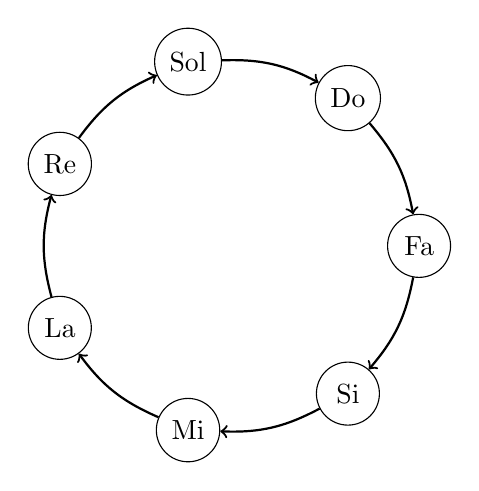
\begin{tikzpicture}[scale=1.2]
		\foreach \note/\angle in {Fa/0, Do/51.43, Sol/102.86, Re/154.29, La/205.71, Mi/257.14, Si/308.57} {
			\node[circle, draw, minimum size=0.8cm] (\note) at (\angle:2cm) {\note};
		}
		\draw[->, thick] (Do) to[bend left=15] (Fa);
		\draw[->, thick] (Fa) to[bend left=15] (Si);
		\draw[->, thick] (Si) to[bend left=15] (Mi);
		\draw[->, thick] (Mi) to[bend left=15] (La);
		\draw[->, thick] (La) to[bend left=15] (Re);
		\draw[->, thick] (Re) to[bend left=15] (Sol);
		\draw[->, thick] (Sol) to[bend left=15] (Do);
	\end{tikzpicture}
	\end{center}

	La progressione per quinte discendenti percorre il cerchio in senso orario. In termini di teoria dei grafi è un \textbf{ciclo hamiltoniano} sul sottografo ciclico delle note diatoniche.

	Con le dodici note, dopo 12 quinte si torna alla nota di partenza: esattamente nel temperamento equabile, a meno del \textit{comma pitagorico} con le quinte pure. Nel sistema diatonico, dopo 7 passi si ritorna alla tonica originale.
\end{matematica}

\begin{matematica}[La struttura ciclica delle progressioni per quinte]
	\label{math:gruppo_z7}
	Le progressioni per quinte discendenti hanno una struttura legata al \textbf{gruppo ciclico} $\mathbb{Z}_7$ (i sette gradi della scala diatonica). Rappresentando i gradi come numeri modulo 7:
	\[
	\text{Gradi: I}=0,\ \text{II}=1,\ \text{III}=2,\ \text{IV}=3,\ \text{V}=4,\ \text{VI}=5,\ \text{VII}=6
	\]

	Un salto di quinta discendente equivale a \textbf{sommare 3 modulo 7} (o sottrarre 4). La progressione completa è:
	\[
	0 \xrightarrow{+3} 3 \xrightarrow{+3} 6 \xrightarrow{+3} 2 \xrightarrow{+3} 5 \xrightarrow{+3} 1 \xrightarrow{+3} 4 \xrightarrow{+3} 0
	\]

	cioè, in gradi:
	\[
	\text{I} \rightarrow \text{IV} \rightarrow \text{VII} \rightarrow \text{III} \rightarrow \text{VI} \rightarrow \text{II} \rightarrow \text{V} \rightarrow \text{I}
	\]

	\begin{itemize}
		\item Dopo 7 passi si torna alla tonica (il gruppo ha ordine 7).
		\item Ogni grado è visitato esattamente una volta ($x \mapsto x+3 \mod 7$ è una permutazione).
		\item L'operazione $+3$ è l'inversa di $-3$ (quinta ascendente): le progressioni per quinte discendenti e ascendenti sono simmetriche.
	\end{itemize}

	Poiché 3 e 7 sono coprimi ($\gcd(3,7) = 1$), $x \mapsto x+3 \mod 7$ genera l'intero gruppo $\mathbb{Z}_7$ e la progressione percorre tutti i gradi prima di tornare alla tonica. Lo stesso vale per le terze discendenti ($-2 \mod 7$, perché $\gcd(2,7) = 1$):
	\[
	0 \xrightarrow{-2} 5 \xrightarrow{-2} 3 \xrightarrow{-2} 1 \xrightarrow{-2} 6 \xrightarrow{-2} 4 \xrightarrow{-2} 2 \xrightarrow{-2} 0
	\]
\end{matematica}

\begin{fisica}[L'energia cinetica delle progressioni ascendenti]
	\label{phys:energia_ascendenti}
	Le progressioni cromatiche ascendenti creano una sensazione di \textbf{accumulo di energia}, per due ragioni. Il movimento verso l'acuto è percepito di per sé come più teso. Inoltre le risoluzioni dissonanza-consonanza sono molto fitte, praticamente una per accordo: ognuna rilascia un poco di tensione, ma subito dopo si presenta una nuova dissonanza, e l'effetto netto è una \textbf{tensione crescente}.
\end{fisica}

\begin{matematica}[Cromatismo e temperamento equabile]
	\label{math:cromatismo_temperamento}
	Le progressioni cromatiche pongono una questione legata al \textbf{temperamento equabile}.

	Nel sistema diatonico puro i semitoni non sono tutti uguali:
	\begin{itemize}
		\item \textbf{semitono cromatico}, per esempio Do-\Dodiesis  (rapporto $\approx 25:24 \approx 1{,}042$);
		\item \textbf{semitono diatonico}, per esempio Mi-Fa (rapporto $\approx 16:15 \approx 1{,}067$).
	\end{itemize}

	In temperamento equabile tutti i semitoni sono identici:
	\[
	\text{Rapporto di semitono} = 2^{1/12} \approx 1{,}059
	\]

	È una media geometrica che rende possibili la modulazione libera e le progressioni cromatiche attraverso tutte le dodici note.

	La progressione cromatica è una \textbf{passeggiata sul gruppo ciclico} $\mathbb{Z}_{12}$: salendo cromaticamente da Do (0),
	\[
	0 \rightarrow 1 \rightarrow 2 \rightarrow 3 \rightarrow 4 \rightarrow 5 \rightarrow 6 \rightarrow 7 \rightarrow 8 \rightarrow 9 \rightarrow 10 \rightarrow 11 \rightarrow 0
	\]
	dopo 12 semitoni si torna esattamente all'ottava superiore. Questa proprietà è garantita solo dal temperamento equabile.

	Nell'intonazione pitagorica (quinte pure 3:2) 12 quinte non tornerebbero esattamente a 7 ottave ma lascerebbero il \textbf{comma pitagorico}:
	\[
	\text{Discrepanza} = \left(\frac{3}{2}\right)^{12} \div 2^7 \approx 1{,}013
	\]

	Il temperamento equabile «distribuisce» l'errore uniformemente su tutti i semitoni e permette la libertà modulatoria e cromatica che caratterizza la musica dal Barocco in poi.
\end{matematica}
